\documentclass[main.tex]{subfiles}
\title{Francesca's Schiacciata focaccia}

\begin{document}

\maketitle% this prints the handout title, author, and date

\begin{abstract}
This is excellent on its own, or used as bread for panini. Focaccia with mortadella, focaccia with any kind of ham, soft cheese, fresh tomato and rocket, are all classics!
\end{abstract}

\begin{marginfigure}%
  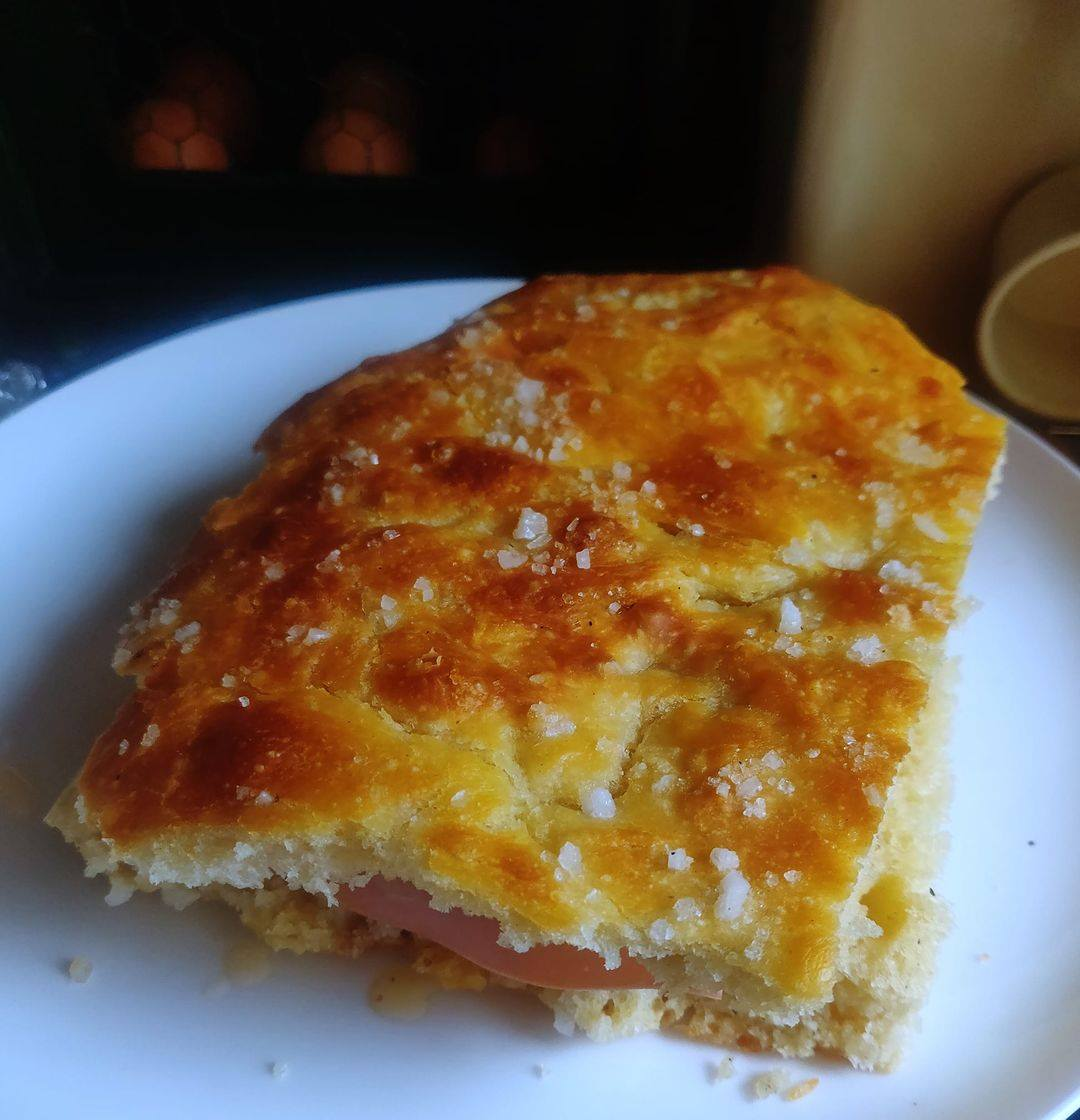
\includegraphics[width=\linewidth]{francesca-focaccia.jpg}
\end{marginfigure}

\section{Ingredients}

\vspace*{-\baselineskip}
\begin{table}[ht]
	\begin{tabularx}{\textwidth}{>{\hsize=0.333\hsize}X>{\bf\hsize=1\hsize}X}
	\unit[500]{g} & bread flour\\
	\unit[7]{g} & dried yeast\\
	\unit[]{} & pinch of salt\\
	\unit[]{} & swirl of oil\\
	\unit[400]{ml} & room temperature water\\
	\end{tabularx}
\end{table}

\section{Instructions}

NOTE: this makes a super wet, hella sticky dough. Work it entirely in a big mixing bowl with a silicon spatula tbh.
\begin{enumerate}
    \item Mix yeast with water and swirl to wake it up.
    \item Mix with flour, salt, oil.
    \item Pour in the water and mix it all up.
    \item Cover the bowl and let rest fifteen minutes.
    \item Knead (with the spatula is less messy) a couple minutes.
    \item Allow to rest 2--3 hours.
    \item Oil the baking dish well, spread the dough in it.
    \item Cover, allow to rest one hour.
    \item Brush with oil, sprinkle with salt.
    \item Bake in hella hot \unit[220--250]{\textdegree C} oven until all cooked.
    \item Depending on oven you may need to turn it upside down to cook through.
\end{enumerate}


% \unit[325]{\textdegree F}

\end{document}

